\lstinputlisting[language=bash,basicstyle=\small]{python_codes/fieldstone_34/keywords.ascii}

\begin{center}
Code at \url{https://github.com/cedrict/fieldstone/tree/master/python_codes/fieldstone_34}
\end{center}

\par\noindent\rule{\textwidth}{0.4pt}

{\sl Exp. 3 of this stone was developed in collaboration with Lukas van de Wiel}.
\index{contributors}{L. van de Wiel}

\par\noindent\rule{\textwidth}{0.4pt}
%%%%%%%%%%%%%%%%%%%%%%%%%%%%%%%%%%%%%%%%%%%%%%%%%%%%%%%%%%%%%%%%%%%%%%%%%%%%%%%%%%%%%%%%%%%%

%---------------------------------------
\subsection*{Experiment 1: Simple shear}

\begin{center}
\includegraphics[width=5cm]{python_codes/fieldstone_34/results/exp1/disp}
\includegraphics[width=5cm]{python_codes/fieldstone_34/results/exp1/p}
\includegraphics[width=5cm]{python_codes/fieldstone_34/results/exp1/exy}
\end{center}


%---------------------------------------
\subsection*{Experiment 2: Pure shear }


\begin{center}
\includegraphics[width=5cm]{python_codes/fieldstone_34/results/exp2/disp}
\includegraphics[width=5cm]{python_codes/fieldstone_34/results/exp2/p}
\end{center}





%---------------------------------------
\subsection*{Experiment 3: Aquarium}

The setup is as follows: a 2D square of elastic material of size $L$ is 
subjected to the following boundary conditions: free slip on the sides, no slip at the 
bottom and free at the top. It has a density $\rho$ and is placed is a gravity 
field ${\vec g}=-g {\vec e}_y$.
For an isotropic elastic medium the stress tensor is given by:
\[
{\bm \sigma} = \lambda ({\vec \nabla}\cdot{\vec \upnu}) {\bm 1} + 2 \mu {\bm \varepsilon}(\vec\upnu)
\]
where $\lambda$ is the Lam{\'e} parameter and $\mu$ is the shear modulus.
The displacement field is ${\vec \upnu}=(0,\upnu_y(y))$ because of symmetry reasons 
(we do not expect any of the dynamic quantities to depend on the $x$ coordinate and 
also expect the horizontal displacement to be exactly zero).
The velocity divergence is then ${\vec \nabla}\cdot{\vec \upnu} = \partial \upnu_y/\partial y$
and the strain tensor:
\[
{\bm \varepsilon}(\vec \upnu)
=
\left(
\begin{array}{cc}
0 & 0 \\
0 & \frac{\partial \upnu_y}{\partial y}
\end{array}
\right)
\]
so that the stress tensor is:

\[
{\bm \sigma} =
\left(
\begin{array}{cc}
\lambda \frac{\partial \upnu_y}{\partial y} &  0 \\
0 & (\lambda + 2 \mu) \frac{\partial \upnu_y}{\partial y}
\end{array}
\right)
\]

\[
{\vec \nabla}\cdot {\bm \sigma} =
(\partial_x \quad \partial_y)\cdot 
\left(
\begin{array}{cc}
\lambda \frac{\partial \upnu_y}{\partial y} &  0 \\
0 & (\lambda + 2 \mu) \frac{\partial \upnu_y}{\partial y}
\end{array}
\right)
=
\left(
\begin{array}{c}
0 \\
(\lambda + 2 \mu) \frac{\partial^2 \upnu_y}{\partial y^2}
\end{array}
\right)
=
\left(
\begin{array}{c}
0 \\
\rho g
\end{array}
\right)
\]
so that the vertical displacement is then given by:
\[
\upnu_y(y) = \frac{1}{2} \frac{\rho g}{\lambda + 2 \mu} y^2 + \alpha y + \beta 
\] 
where $\alpha$ and $\beta$ are two integration constants.
We need now to use the two boundary conditions: the first one states that the displacement
is zero at the bottom, i.e. $u_y(y=0)=0$ which immediately implies $\beta=0$.
The second states that the stress at the top is zero (free surface), which implies that 
$\partial u_y/\partial y (y=L)=0$ which allows us to compute $\alpha$.
Finally:
\[
u_y(y) = \frac{\rho g}{\lambda + 2 \mu} (\frac{y^2}{2}-L y) 
\] 
The pressure is given by
\[
p=-(\lambda + \frac{2}{3} \mu) {\vec \nabla}\cdot{\vec\upnu}
= (\lambda + \frac{2}{3} \mu)  \frac{\rho g}{\lambda + 2 \mu} (L -y)
= \frac{\lambda + \frac{2}{3} \mu}{\lambda + 2 \mu} \rho g (L-y)  
= \frac{1 + \frac{2 \mu}{3 \lambda} }{1 + 2 \mu/\lambda} \rho g (L-y)  
\]
In the incompressible limit, the poisson ratio is $\nu \sim 0.5$. 
Materials are characterised by a finite Young's modulus $E$, which is related to 
$\nu$ and $\lambda$:
\[
\lambda=\frac{E \nu}{(1+\nu)(1-2\nu)}
\quad\quad
\mu=\frac{E}{2(1+\nu)}
\]
It is then clear that for incompressible parameters $\lambda$ becomes 
infinite while $\mu$ remains finite. In that case the pressure 
then logically converges to the well known formula:
\[
p=\rho g (L-y)
\]

In what follows we set $L=1000$m, $\rho=2800$, $\nu=0.25$, $E=6\cdot10^{10}$, $g=9.81$.

\begin{center}
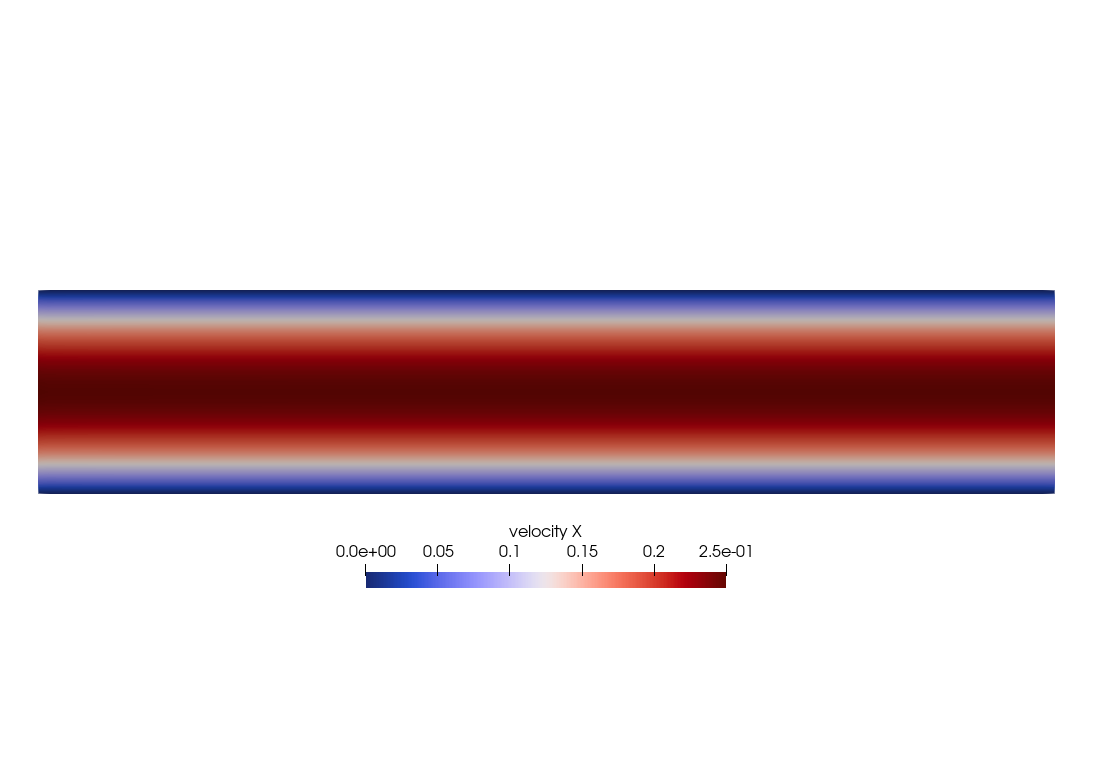
\includegraphics[width=5cm]{python_codes/fieldstone_34/results/exp3/u}
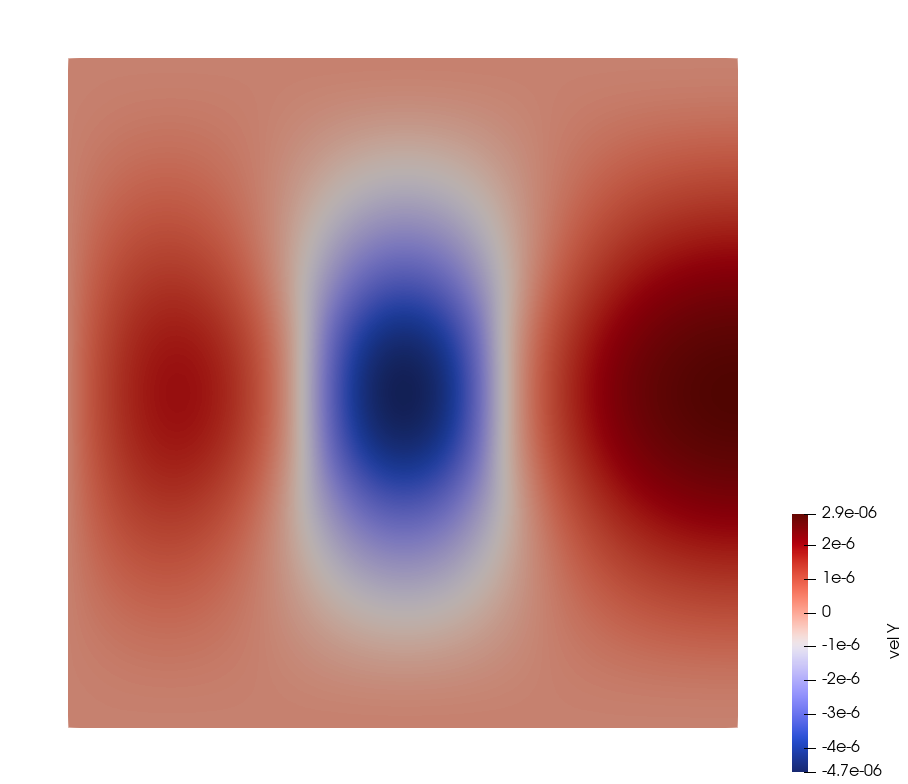
\includegraphics[width=5cm]{python_codes/fieldstone_34/results/exp3/v}
\includegraphics[width=5cm]{python_codes/fieldstone_34/results/exp3/p}\\
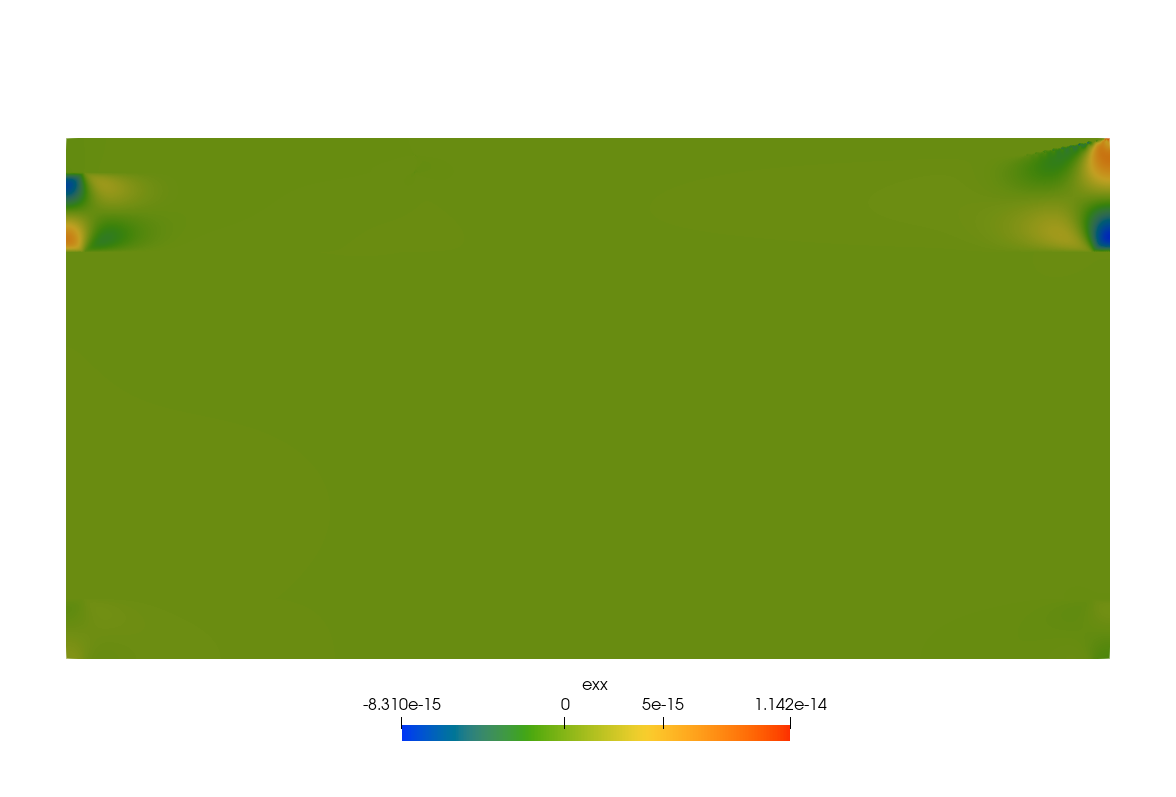
\includegraphics[width=5cm]{python_codes/fieldstone_34/results/exp3/exx}
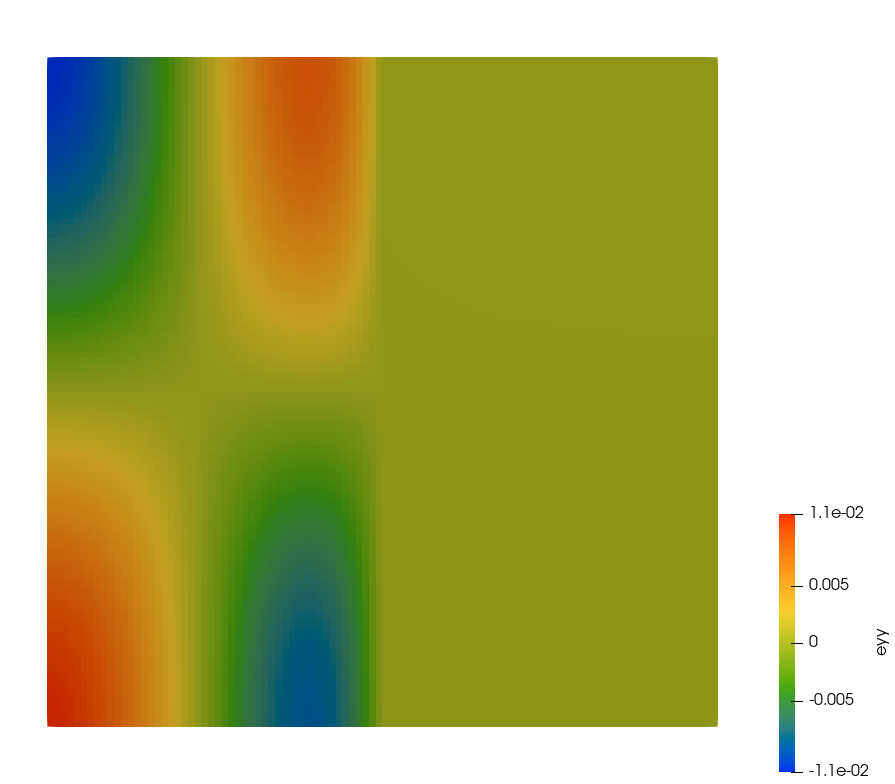
\includegraphics[width=5cm]{python_codes/fieldstone_34/results/exp3/eyy}
\includegraphics[width=5cm]{python_codes/fieldstone_34/results/exp3/exy}
\end{center}

\begin{center}
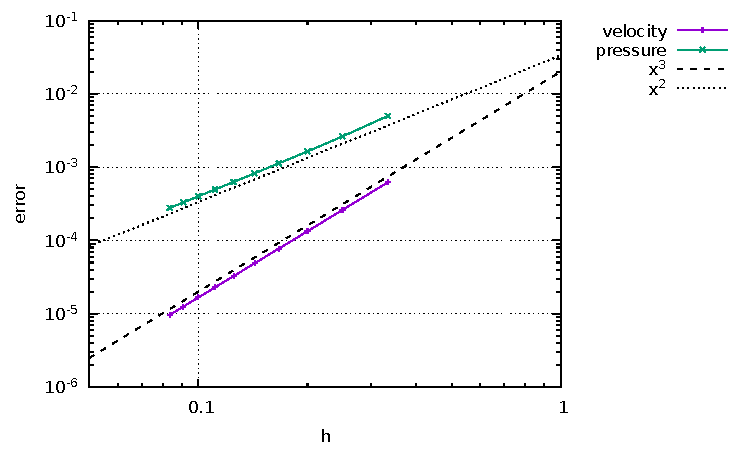
\includegraphics[width=12cm]{python_codes/fieldstone_34/results/exp3/errors.pdf}
\end{center}


%---------------------------------------
\subsection*{Experiment 4: Strip load}

The domain is $3 \times 2~\si{\km}$. Free slip boundary conditions are 
applied on the sides and bottom boundaries. 
Traction boundaries corresponding to a pressure of $\SI{100}{\mega\pascal}$
are prescribed on the top boundaries for $|x-L_x/2|<a$ with $a=\SI{50}{\meter}$.
Material parameters are identical to those of experiment 3.

\begin{center}
\includegraphics[width=5cm]{python_codes/fieldstone_34/images/dase96a}
\includegraphics[width=5cm]{python_codes/fieldstone_34/images/dase96b}
\includegraphics[width=5cm]{python_codes/fieldstone_34/images/dase96c}
\end{center}


The analytical solution is given in terms of the stress tensor.
From \textcite{dase96}(section 4.6) we have the components of the stress tensor:
\[
\sigma_{xx}=\frac{p_0}{\pi}\left[ \theta - \frac{1}{2}\sin 2\theta  \right]^{\theta_2}_{\theta_1}
\quad\quad\quad
\sigma_{zz}=\frac{p_0}{\pi}\left[ \theta + \frac{1}{2}\sin 2\theta  \right]^{\theta_2}_{\theta_1}
\quad\quad\quad
\sigma_{xz}=\frac{p_0}{\pi}\left[ \sin^2 \theta  \right]^{\theta_2}_{\theta_1}
\]
or, 
\begin{eqnarray}
{\sigma}_{xx}&=&\frac{p_0}{\pi}\left[ \theta - \frac{1}{2}\sin 2\theta  \right]^{\theta_2}_{\theta_1} = \Theta - \frac{1}{2} ( \sin 2\theta_2 - \sin 2\theta_1) \nn\\
{\sigma}_{zz}&=&\frac{p_0}{\pi}\left[ \theta + \frac{1}{2}\sin 2\theta  \right]^{\theta_2}_{\theta_1} = \Theta + \frac{1}{2} ( \sin 2\theta_2 - \sin 2\theta_1) \nn\\
{\sigma}_{xz}&=&\frac{p_0}{\pi}\left[ \sin^2 \theta  \right]^{\theta_2}_{\theta_1} =  \sin^2 \theta_2 - \sin^2 \theta_1 \nn
\end{eqnarray}
with $\Theta=\theta_2-\theta_1$. 

\begin{center}
\includegraphics[width=5.7cm]{python_codes/fieldstone_34/results/exp4/disp}\\
\includegraphics[width=5.7cm]{python_codes/fieldstone_34/results/exp4/sigma_xx}
\includegraphics[width=5.7cm]{python_codes/fieldstone_34/results/exp4/sigma_yy}
\includegraphics[width=5.7cm]{python_codes/fieldstone_34/results/exp4/sigma_xy}\\
\includegraphics[width=5.7cm]{python_codes/fieldstone_34/results/exp4/sigma_xx_th}
\includegraphics[width=5.7cm]{python_codes/fieldstone_34/results/exp4/sigma_yy_th}
\includegraphics[width=5.7cm]{python_codes/fieldstone_34/results/exp4/sigma_xy_th}\\
{\captionfont Results obtained on 300x200 mesh. Top row is recovered stresses. 
Bottom row is analytical solution.}
\end{center}

